%
% snellius.tex -- Brechungsgesetz
%
% (c) 2019 Prof Dr Andreas Müller, Hochschule Rapperswil
%
\documentclass[tikz,12pt]{standalone}
\usepackage{times}
\usepackage{amsmath}
\usepackage{txfonts}
\usepackage[utf8]{inputenc}
\usepackage{graphics}
\usepackage{color}
\usepackage{pifont}
\usetikzlibrary{arrows,intersections,math,calc}
\begin{document}

\def\punkt#1{
        \fill[color=white] #1 circle[radius=0.08];
        \draw #1 circle[radius=0.08];
}

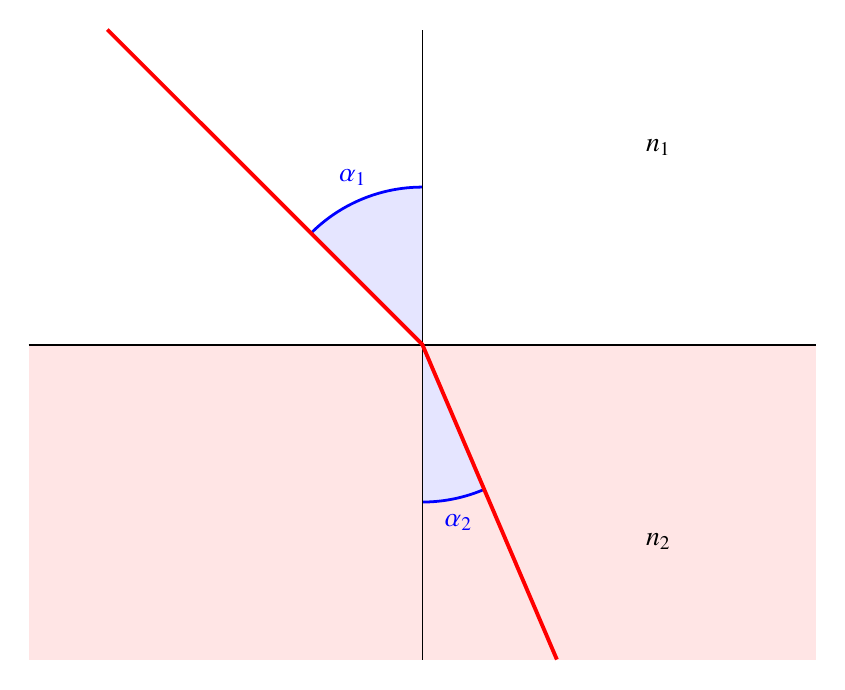
\begin{tikzpicture}[>=latex,thick]

\def\h{4}
\def\w{5}

\fill[color=red!10] ({-\w},0)--({-\w},-{\h})--({\w},{-\h})--({\w},0)--cycle;

\def\none{1}
\def\none{1.8}

\def\a{45}
\def\b{23.1311}

\fill[color=blue!10] (0,2) arc (90:{90+\a}:2) -- (0,0)--cycle;
\draw[line width=1pt,color=blue] (0,2) arc (90:{90+\a}:2);

\node[color=blue] at ({-2.3*sin(\a/2)},{2.3*cos(\a/2)}) {$\alpha_1$};
\node[color=blue] at ({2.3*sin(\b/2)},{-2.3*cos(\b/2)}) {$\alpha_2$};

\fill[color=blue!10] (0,-2) arc (270:{270+\b}:2) -- (0,0)--cycle;
\draw[line width=1pt,color=blue] (0,-2) arc (270:{270+\b}:2);

\draw[line width=0.7pt] ({-\w},0)--({\w},0);
\draw[line width=0.5pt] (0,{-\h})--(0,{\h});

\draw[line width=1.4pt,color=red]
	({-\h*sin(\a)/cos(\a)},\h)--(0,0)--({\h*sin(\b)/cos(\b)},-\h);

\node at (3,2.5) {$n_1$};
\node at (3,-2.5) {$n_2$};

\end{tikzpicture}

\end{document}

